\documentclass[../index.tex]{subfiles}

\begin{document}
У світі фінансів і торгівлі цінними паперами, централізовані біржі завжди
відігравали ключову роль, забезпечуючи надійність та безпеку черезе
централізовану інфраструктуру для трейдерів та інвесторів. Проте останнім часом
відбувається зростання інтересу до децентралізованих бірж, що призводить до
переворотних змін у фінансовому секторі. Децентралізовані біржі стають ключовим
елементом цієї нової економічної парадигми. Підкріпленні математикою та
детермінованими правилами, децентралізовані біржі забезпечують прозорість та
надійність для їх користвачів, що дає поля для розвитку нових незалежних гравців
ринку.

У данній роботі ми розглядаємо біржі основані на методі автоматизованих
маркет-мейкерів (з англ. ``Automated Market Maker'') найдавніша згадка котрих
датується ще 1956~\cite{mccarthy}. Конкретно розглянемо простий для аналізу і
один з найпопулярніших по кількості імплементацій варіант на константних
функціях~\cite{angeris_2023}.

На відміну від традиційних бірж, де ціна визначається за допомогою зіставлення
заявок купівлі та продажу, ААМ використовують алгоритм для визначення відношення
вартості валют через кількості вкладів (ліквідність) у валютну пару. Це дозволяє
створити вигідну систему для владників ліквідності, що отримують винагороду за
свої вклади, та трейдерів, що бажають скористатися платформою і ліквідністю
вкладників для обміну.

Також основною цілю нашого дослідженню буде біржа
UniswapV2~\cite{adams2021uniswap}, котра є однією з найпопуляніших імплементацій
АММ на даний момент.

\subsection{Константна функція обміну}\label{sec:math-model}

ММКФ відносно просто описати аналітично, тому багато дослідників і практиків
працюють з ними саме в такому ``аналітичному'' середовищі. Модель складається з
двох основних об'єктів: торгової функції (надалі функція обміну)
$f : \mathbf{R}_{+}^{n} \mapsto \mathbf{R}$ та вектора запасів
$R \in \mathbf{R}^{n}_{+}$. Користувач пропонує обмін, представлений у вигляді
портфеля $\Delta \in \mathbf{R}_{n}$, і обмін вважається дійсним, якщо торгова
функція, оцінена на резервах після завершення обміну, має те саме значення, що і
функція, оцінена на резервах до завершення угоди, тобто, якщо
$f(R - \Delta) = f(R)$. (Звідси і назва ``маркет-мейкер з постійною функцією''.)
Якщо ця рівність виконується, то ММКФ виплачує користувачеві $\Delta$, що
призводить до появи нових резервів $R - \Delta$. (Якщо угода є недійсною,
користувач нічого не отримує і не виплачує.) Постачальники ліквідності, які
надають резерви $R$, під які здійснюються угоди, заробляють на цих угодах
комісійні. Той факт, що цей процес легко описати і реалізувати, а також те, що
він має багато сильних теоретичних гарантій, став однією з причин його успіху,
особливо в таких складних для захисту середовищах, як публічні блокчейни.
Незважаючи на простий опис, ММКФ породили велику кількість досліджень їх
фінансових, арбітражних і маршрутних властивостей
(наприклад,~\cite{Angeris_2020},~\cite{danos}, серед багатьох інших).

У нашому випадку розглядається імлементація ММКФ від Uniswap:

\begin{equation}\label{eq:intro-swap}
	R_{X} \cdot R_{Y} = k = const
\end{equation}

де \(R_{X}\) кількість валюти (резерви від англ. ``reserves'') \(X\), та
\(R_{Y}\) кількість валюти \(Y\) у парі \(X/Y\), а \(k\) --- деяка константа котра
задається при створенні пари на біржі. Що є маркет мейкером константного
добутку~\cite{zhang2018formal} (з англ. \textit{``CPMM Constant Product Market
  Maker''}), де відношення вкладів до і після має бути константним. Тобто при
продажі $\Delta x$ валюти отримуємо $\Delta y$:

\begin{equation*}
	R_{X} \cdot R_{Y} = (R_{X} + \Delta x) \cdot (R_{Y} - \Delta y)
\end{equation*}

\begin{figure}[h!]
	\centering
	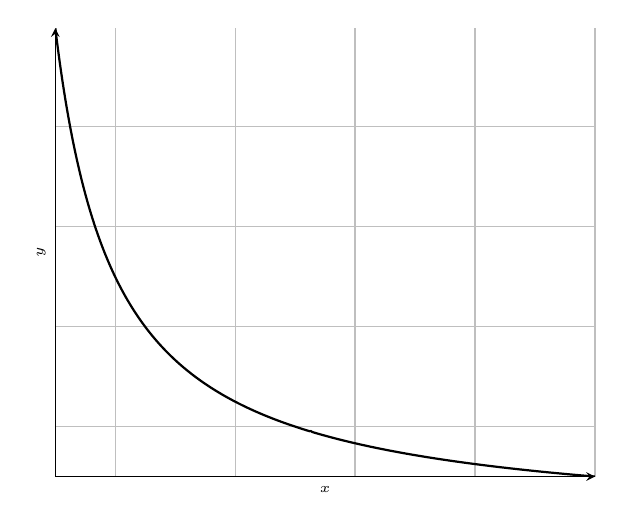
\begin{tikzpicture}[domain=0:4]
		\begin{axis}%
			[
				grid=major,
				ticks=none,
				xlabel={\tiny $x$},
				ylabel={\tiny $y$},
				axis x line=left,
				axis y line=left,
				no markers,
				domain=0:10,
				restrict y to domain=0:10000
			]
			\addplot[thick,samples=400] (x,{10000/x});
		\end{axis}
	\end{tikzpicture}
	\caption{Зображення графіку залежностей вкладів у пару}\label{fig:isoquant}
\end{figure}

\subsection{Біржевий граф}

Нехай \(G_{t} = (V_{t}, E_{t})\) --- неорієнтований динамічний граф, де \(V_{t}\) ---
множина вершин таких, що кожна вершина є конкретною валютою на біржі,
\(E_{t}\) --- множина ребер цього графа, тобто кожне ребро відображує те, чи є
можливість на біржі обміняти деякі дві різні валюти з \(V_{t}\), у момент часу
\(t\).

Так як в залежності від часу на біржі можуть з'являтися та зникати як валюти так
і зв'язки (шляхи обміну) між ними, то ми описуємо біржу у вигляді динамічного
графа, що залежить від часу \(t\)~\cite{siljak}. Вага ребра визначається як
функція від вкладів у пару на момент часу \(t\) та об'єму обміну при проходженні
через дане ребро (про що мова йде далі).

У біржі існує два типи подій, що змінюють стан біржі:

\begin{enumerate}
  \item Створення нової пари (змінює ребра та вершини).
  \item Обмін однієї пари або послідовності валют на біржі (змінює ваги ребер).
\end{enumerate}
\end{document}
